\documentclass{report}
\author{Benjamin Isenhart}
\usepackage[width=150mm,top=25mm,bottom=25mm]{geometry}
\usepackage{setspace}
\doublespacing
\usepackage{graphicx}
\usepackage{wrapfig}
\usepackage{physics}
\usepackage{fancyhdr}
\pagestyle{fancy}

\begin{document}


\begin{titlepage}
	\begin{center}
		\vspace{1cm}
		\Huge
		\textbf{Precise Control of Organic LED Emission Through Optically Resonant Microcavity Amplification}\\
		\vspace{1.5cm}
		\Large
		An Honors Thesis Presented\\
		by\\
		Benjamin Isenhart\\
		to\\
		The Faculty of the University of Vermont\\
		\vspace{0.5cm}
		Spring 2019
		\vspace{2cm}
	\end{center}
	\begin{flushright}
		\Large
		Defense Date: 2nd May, 2019\\
		Thesis Examination Committee:\\
		\vspace{0.5cm}
		Frederic Sansoz, Ph.D., Chairperson\\
		Matthew S. White, Ph.D., Advisor\\
		Madalina Furis, Ph.D.\\
	\end{flushright}
\end{titlepage}

\chapter*{Abstract} \label{abstract}
The ability to change the emission spectrum of an LED device has traditionally only been possible through chemical changes to the emissive material or the addition of dopants. Both of these techniques have significant disadvantages due to the limited range of changes possible and the difficulty of precisely controlling these changes. We present a technique of precisely controlling the emission spectrum of a device through device design alone. By placing reflective electrodes on either side of an LED device, we generate an optically resonant microcavity whose properties impact the emission profile of the device. The direct relationship between the cavity thickness and the peak emission wavelength allows for tuning of the peak emission to within the resolution of our ability to deposit films. We additionally explore the impacts of stacking multiple microcavities on top of one another in the emission profile.

\tableofcontents

\chapter{Introduction} \label{intro}

    \section{Organic Light Emitting Diodes}
        Light emitting diodes (LEDs) have become prevalent in everyday life in applications ranging from screens to the headlights on cars. They have widely replaced the more traditional incandescent bulbs due to increased power efficiency, longevity, and compact size when compared to other luminescent devices. However, the most common LEDs require hazardous semiconductors such as gallium and arsenic doped silicon (CITE). In order to mitigate this, LEDs based off of organic materials, called OLEDs, have come into fruition. OLEDs are usually comprised of a transparent conductive oxide (TCO) as a transparent electrode, a metal for the non-transparent electrode, and three organic materials. These organic materials are used as a hole transport material, electron transport material, and an emissive material. The emissive material has a band structure suitable for electron and hole recombination and the release of a photon in the visible spectrum. The hole and electron transport materials serve primarily to ensure that all electron-hole recombination occurs in the emissive material (CITE?).
        
    \section{Waveguides and the Fabry-P\'erot Etalon}
        \begin{figure}
            \centering
            
\includegraphics[width=0.75\textwidth]{images/etalon_schematic.png}
            \caption{Schematic of the Fabry-P\'erot etalon. The steady state solutions for wave propogation in the etalon are shown. Credit: (CITE DOI:10.1364/OE.24.016366)}
            \label{fig:etalon}
        \end{figure}

        In electomagnetism, a waveguide is defined as a surface or set of surfaces made of a conductor such that the electric and magnetic fields within the conductor are restricted to zero. These waveguides provide boundary conditions to Maxwell's equations, such that only specific modes of propogation can occur within the waveguide. These allowed modes are generally called the transverse electric (TE) mode, the transverse magnetic (TM) mode, and in the special case of both TE and TM, the TEM mode (CITE GRIFFITHS). One special form of waveguide, called the Fabry-P\'erot etalon, is characterized by two conducting planes with a transparent material in between (CITE). Due to the structure of the etalon, certain wavelengths of light resonate and are amplified by the etalon, while others destructively interfere with their reflections, and are eliminated. In particular, the condition for amplification is that the frequency $\nu$ and wavenumber $k$ obey:
        \begin{equation}
            \nu_q=\frac{qc}{2ln}\ \mathrm{and}\ k_q=\frac{\pi q}{l}
        \end{equation}
        for the $q$th resonant mode. Here $c$ is the speed of light in vacuum, $l$ is the geometric length of the etalon, and $n$ is the index of refraction for the material inside (CITE DOI:10.1364/OL.43.005033). In the case of light propogating normal to the two planes, this condition can be intuitively understood as standing waves that have no amplitude at the metal surfaces. The amplification of light through the Fabry-P\'erot etalon is given by:
        \begin{equation}
            A'_{trans}=\frac{I_{trans}}{I_{inc}}=\frac{\qty(1-R_1)\qty(1-R_2)}{\qty(1-\sqrt{R_1R_2})^2+4\sqrt{R_1R_2}\sin^2(\phi)}
        \end{equation}
        where $\phi$ describes the phase shift between forward and backward propogating waves. In the special case of the resonant mode, $\phi=0$, so the resonant mode amplification is given by:
        \begin{equation}
            A'_{trans}\qty(\nu_q)=\frac{\qty(1-R_1)\qty(1-R_2)}{\qty(1-\sqrt{R_1R_2})^2}
        \end{equation}
        where $R_1$ and $R_2$ are the reflectivities of the conductive planes (CITE SIEGMAN).
        
    \section{OLEDs in Optically Resonant Microcavities}
        In the traditional Fabry-P\'erot etalon, the light source is located outside of the conductor planes, and the spectrum is collected on the opposite side of the conductor planes. However, by replacing the transparent electrode in an OLED with a partially reflective, partially transparent conductor, the electrodes of the device can be used as two reflective planes, making a Fabry-P\'erot etalon with the light source between the reflective planes. This can be achieved with a thin metal film as the partially transparent electrode. In this project, devices of this form were fabricated so that the emission of the OLED device underwent amplification by this optically resonant microcavity and the dependence of the emission spectrum on physical propoerties of the microcavity were explored.

\chapter{Experimental Methods} \label{methods}

    \section{OLED Materials} \label{materials}
    An tris-(8-hydroxyquinoline)aluminum (Alq$_3$) emissive material, along with bathophenanthroline (BPhen) as an electron transport material and N,N′-Di(1-naphthyl)-N,N′-diphenyl-(1,1′-biphenyl)-4,4′-diamine (NPB) as a hole transport material, were chosen due to their reported use in a green OLED devices by (CITE doi:10.1063/1.3634210). Silver and molibdinum oxide (Ag/MoO$_3$) were used for the hole selective electrode, while aluminum and lithium flouride (Al/LiF) were used for the electron selective electrode. The organics were purchased from Sigma-Aldrich and purified through sublimation.\\
    \begin{figure}[h!]
        \centering
        (a)
        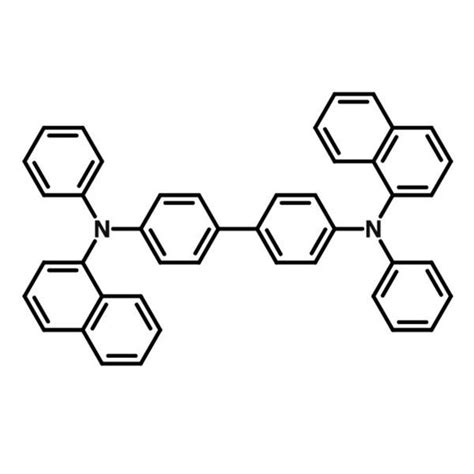
\includegraphics[width=0.29\textwidth]{images/npb_structure.jpg}
        (b)
        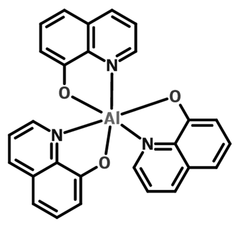
\includegraphics[width=0.29\textwidth]{images/alq3_structure.png}
        (c)
        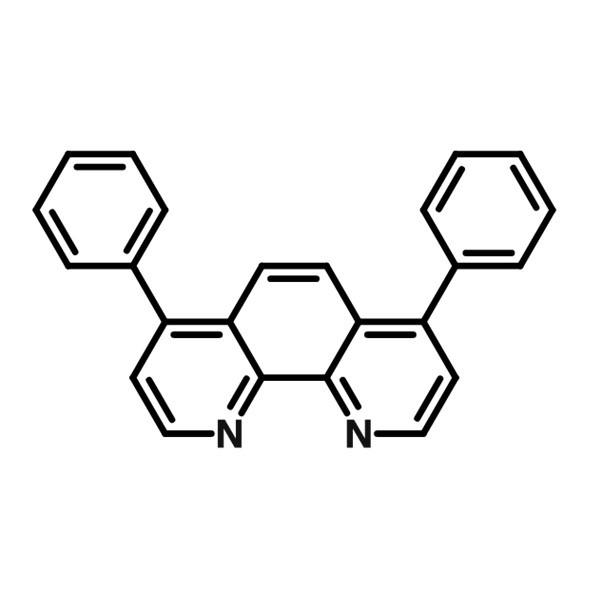
\includegraphics[width=0.29\textwidth]{images/bphen_structure.jpg}
        \caption{Chemical structures of (a) the NPB hole transport material, (b) the Alq$_3$ emitter material, and (c) the BPhen electron transport material.}
        \label{fig:structures}
    \end{figure}
    \newpage

    \section{Device Fabrication} \label{fab}
    \begin{wrapfigure}{r}{0.4\textwidth}
        \centering
        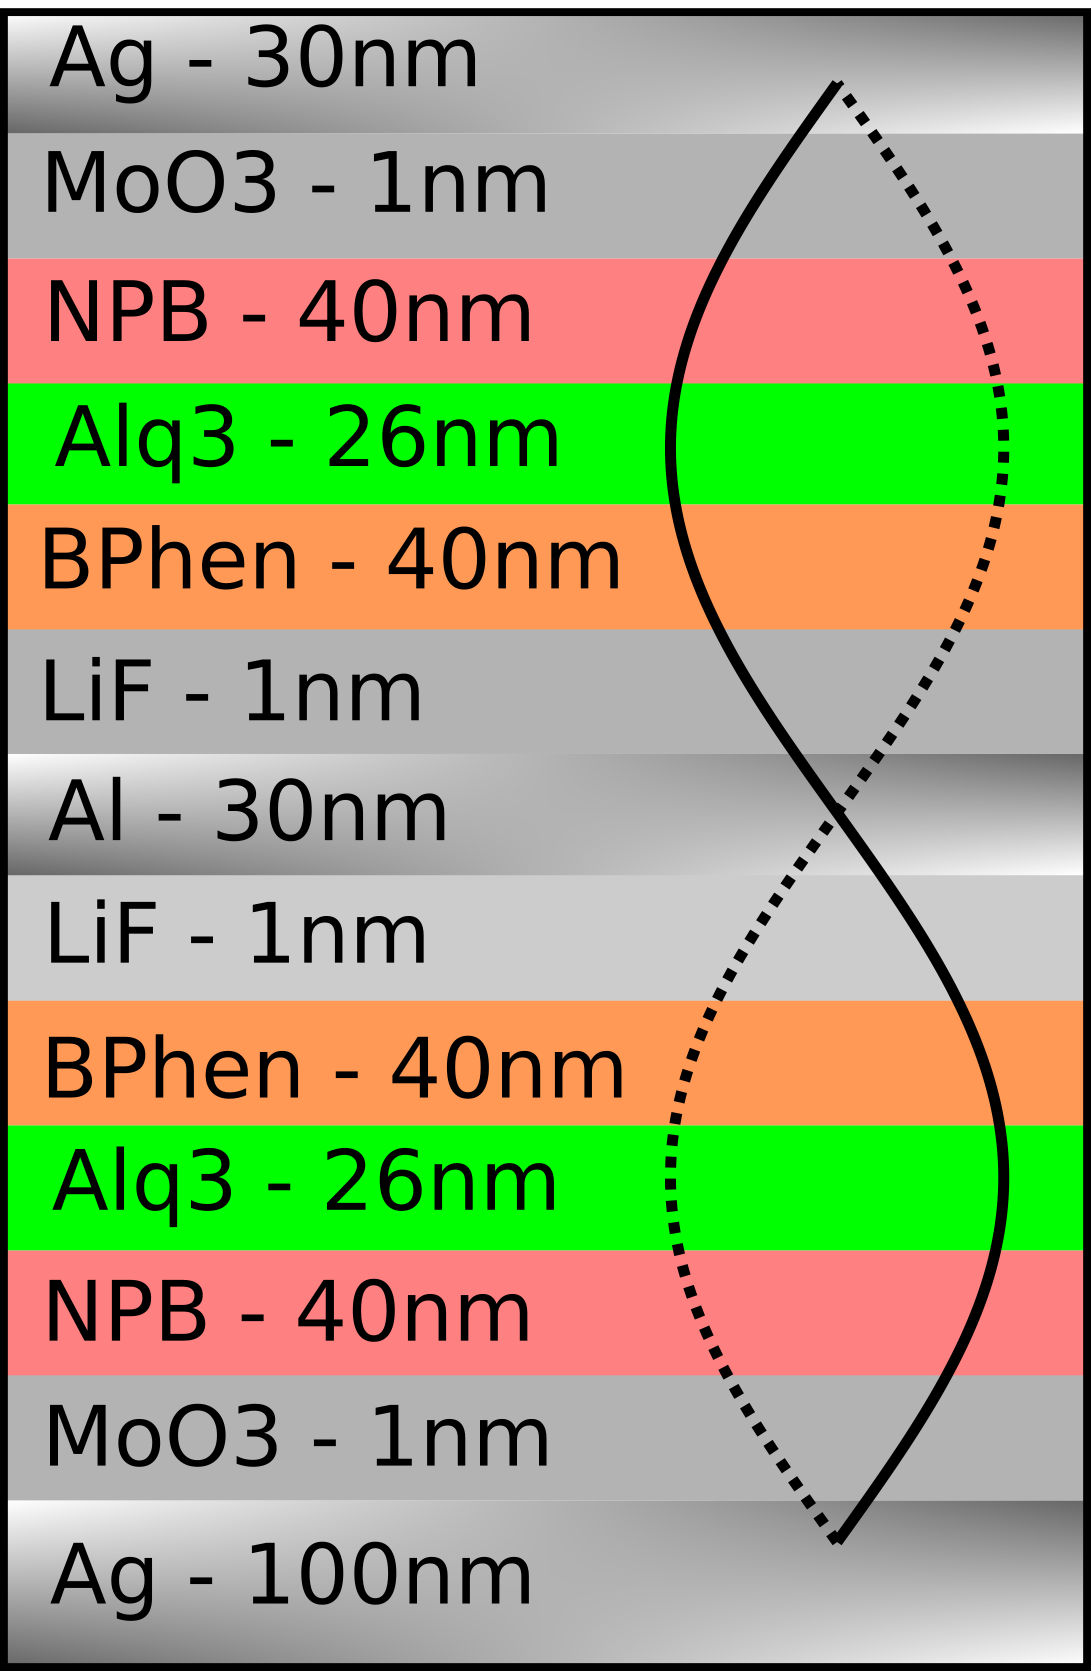
\includegraphics[width=0.3\textwidth]{images/schematic.png}
        \caption{\small Schematic of a two-cavity device and the $\lambda/2$ resonant mode.}
        \label{fig:schematic}
    \end{wrapfigure}
    In order to generate optically resonant microcavities, a standard OLED recipe was used (CITE) with the substitution of a 30nm metal electrode in the place of a transparent electrode. In particular, an oxidized silicon substrate had a 100nm bottom electrode of silver, followed by 1nm of molibdinum oxide, $x$nm of NPB, 20 (single cavity devices) or 26nm (multi-caqvity devices) of Alq$_3$, $x$nm of BPhen, 1nm of lithium flouride, and 30nm of aluminum deposited onto it through sequential thermal evaporation. For multi-cavity devices, this same structure was replicated in the following cavity, but inverted, as shown in Figure \ref{fig:schematic}. The thickness $x$ of the NPB and BPhen layers was modified to generate whatever cavity thickness was desired. In all multi-cavity devices transport layer thicknesses of $x=40$nm were used. All depositions were performed under a pressure of $10^{-7}$torr and vacuum was not broken during processing.

    \section{Emission Spectroscopy} \label{spect}
    Devices were stored and tested in a nitrogen glovebox with $<0.01$ppm O$_2$ and $<0.05$ppm H$_2$O to avoid degradation of devices. Emission spectra were collected using an OceanOptics (NAME?) spectrometer with a fiberoptic passthrough to the glovebox. The emission of the devices was passed through an iris to minimize the collection angle, then reflected off of a parabolic mirror to focus the emission into the fiber. Devices were mounted on a rotating stage and emission spectra were collected at 2.5 degree intervals from 0 to 90 degrees.

\chapter{Results}

    \section{Single Cavity Devices} \label{n=1}

        In all single cavity devices, a 100nm bottom electrode was used with a 30nm top electrode to produce a resonant cavity of the desired size. The thickness of the organics was changed in order to maintain a 20nm Alq$_3$ layer between the contact layers. In all devices except those described in section \ref{topMaterial}, a silver electrode with a MoO$_3$ cap was used as the bottom electrode and an aluminum electrode with a LiF cap was used for the top.
    
        \begin{figure}[h!]%{r}{0.55\textwidth}
            \centering
            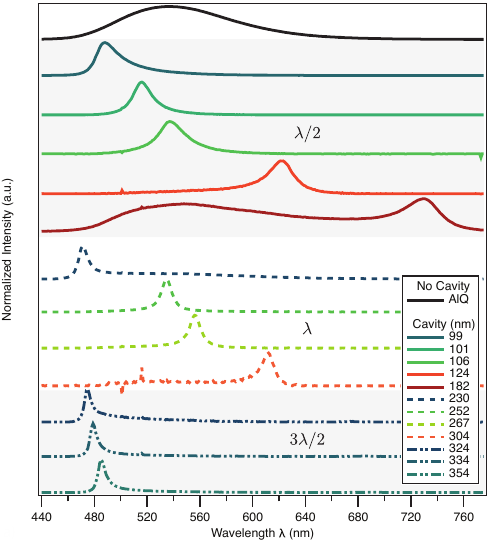
\includegraphics[width=0.75\textwidth]{images/n1_spectra.png}
            \caption{Emission spectra of single cavity devices of various cavity thicknesses, along with the natural emission spectrum of the Alq$_3$ emitter. As cavity thickness increases, the emission peak redshifts, until it shifts to the next resonant mode, returning to a blue color. Following each shift to the next resonant mode, the bandwidth of the emission narrows. The 182nm device shows a strong broadband emission along with the resonant mode. That is because the natural emission at the wavelength of the resonant mode is extremely weak, so the broadband leakage out of the cavity is on the same order as the resonant emission.}
            \label{fig:n1_spectra}
        \end{figure}
        
%        \begin{figure}
%             \centering
%             \vspace{-1cm}
%             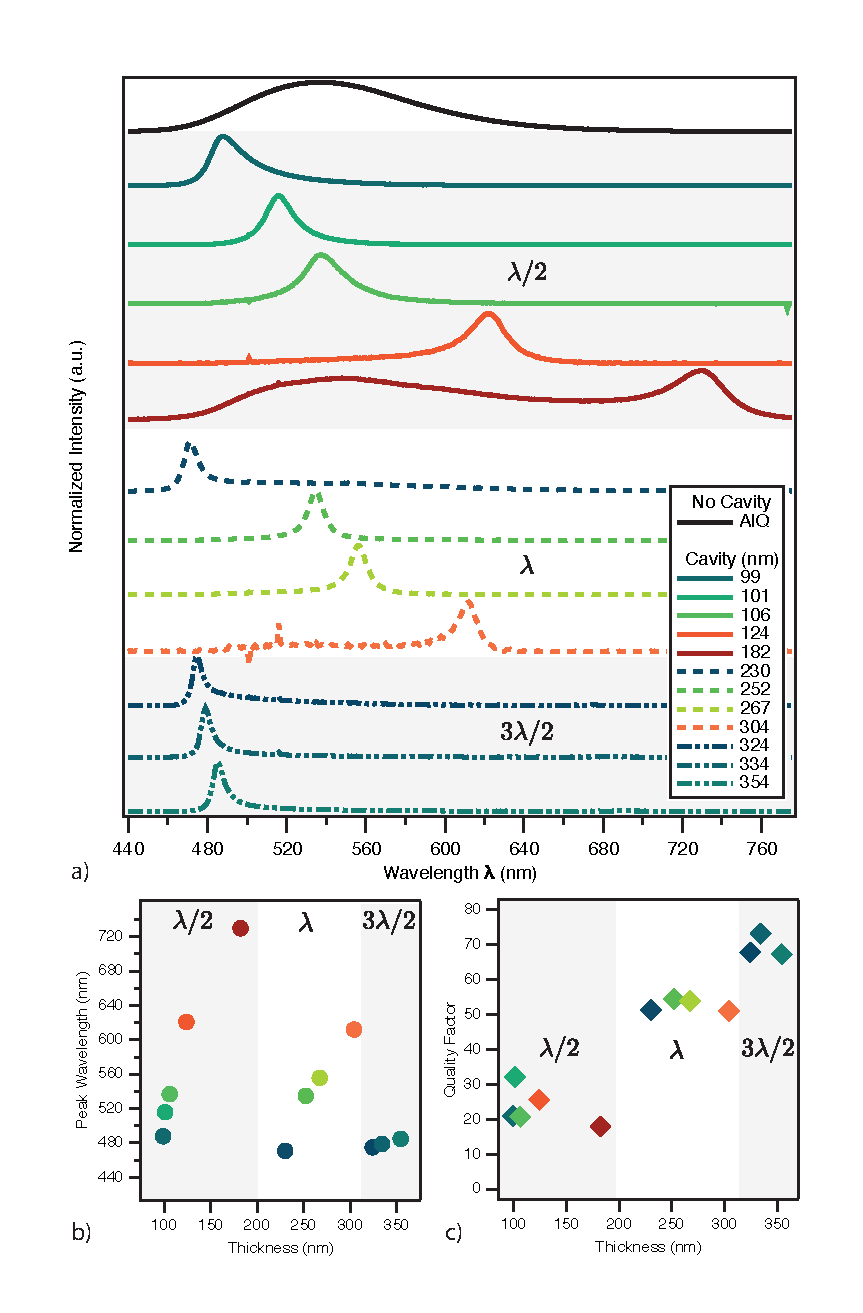
\includegraphics[width=0.99\textwidth]{images/n1_overview.pdf}
%             \vspace{-1cm}
%             \caption{Emission characteristics of single cavity devices:\newline (a): Emission spectrum as a function of cavity thickness\newline (b): Peak wavelength as a function of cavity thickness,\newline (c): Quality factor as a function of cavity thickness}
%         \end{figure}

    
        \subsection{Peak Emission Wavelength} \label{peakWavelength}
            \begin{wrapfigure}{r}{0.45\textwidth}
                \centering
                \vspace{-1cm}
                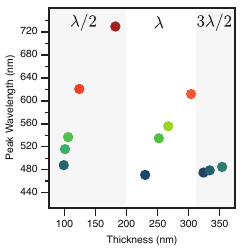
\includegraphics[width=0.4\textwidth]{images/n1_peak_emission.png}
                \caption{\small Peak emission wavelength as a function of thickness for various single cavity devices.}
                \label{fig:peak_emission}
            \end{wrapfigure}

            An analysis of the peak wavelength of emission for each cavity thickness reveals a very strong correlation. In particular, a linear relationship is observed between the peak wavelength and the resonance cavity thickness, as shown in Figure \ref{fig:peak_emission}. This is logical as the wavelength of a resonant mode should be proportional to the width of the resonance cavity, with the constant of proportionality being the index of refraction for light in the organic materials. We do see some variation from the linear model, which is to be expected the overall index of refraction in the cavity is not a constant across devices. Specifically, by not keeping the ratio of each organics layer the same, we inadvertantly modified the index of refraction slightly, leading to small variations from the linear model.
            
            The linear model, however, is only valid for the regime of a single resonant mode. We see a break in the linearity of peak emission wavelength and cavity thicknesses at the points of transition from a half-integer resonance to the next. we have measured the transition from $\lambda/2$ to $\lambda$ and from $\lambda$ to $3\lambda/2$ at approximately 200nm and 310nm, respectively. This is as expected, as the resonant wavelength doubles when shifting from one half-integer mode to the next. We also notice that when the linear relationship picks up again on the other side of a transition to the next mode, the slope is decreased by a factor of roughly two, indicating that the constant of proportionality discussed above is not just dependent on the index of refraction, but also which resonant mode is being described.
        
        \subsection{Band Narrowing} \label{bandwidth}
            \begin{wrapfigure}{r}{0.45\textwidth}
                \centering
                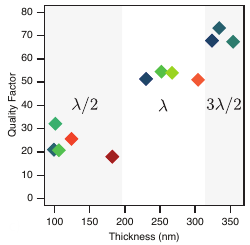
\includegraphics[width=0.4\textwidth]{images/n1_quality_factor.png}
                \caption{\small Quality factor as a function of cavity thickness for various single cavity devices.}
                \label{fig:bandwidth}
            \end{wrapfigure}

            Analysis of the quality factor (EXPLAIN?) shows that it also has a linear relationship with the cavity thickness as shown in Figure \ref{fig:bandwidth}. Unlike the peak emission wavelength, the linearity of the quality factor does not break at the transitions between resonant modes. This correlation can be understood as a manifestation of the Heisenberg uncertainty principle (CITE). In particular, as we widen the cavity, we increase the uncertainty in the position of a photon in the cavity. This increased uncertainty in the position of the photon gives us the ability to more precisely determine its momentum, which is directly proportional to its wavelength. Thus, the spread of wavelengths can be shrunk, effectively narrowing the bandwidth of the resonant emission.

            We do see a strong outlier to the linear model in the 182nm cavity device. The quality factor of this device is significantly lower than would be expected with the linear model presented above. However, a look at the emission spectrum of this device makes the cause of this very clear (REFERENCE IMAGE). The resonant mode of this device has a wavelength of approximately 730nm, which is very far outside of the natural emission of the Alq$_3$ emitter. The emission spectrum shows that the emission of the resonant mode is on the same order as the broadband leakage out of the cavity. Thus, the calculation of the quality factor for the resonant mode is skewed due to the broadband emission widening the emission peak.
        
        \subsection{Effect of Top Electrode Material} \label{topMaterial}
            \begin{figure}[h!]
                \centering
                (a)
                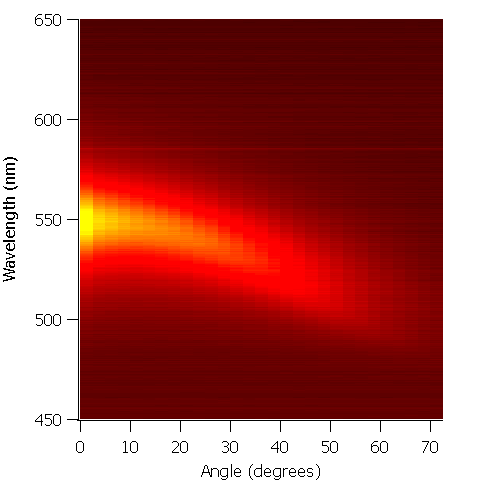
\includegraphics[width=0.45\textwidth]{images/n1_ag_top_heatmap.png}
                (b)
                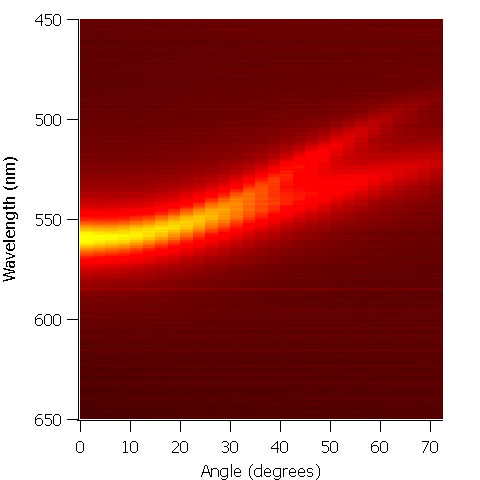
\includegraphics[width=0.45\textwidth]{images/n1_al_top_heatmap.png}
                \caption{\small Angular resolved emission profiles of single cavity devices topped with a silver electrode (a), and with an aluminum electrode (b). The aluminum topped device shows a much narrower emission peak than the silver topped device due to differences in optical properties of the metals.}
                \label{fig:topMaterial}
            \end{figure}

            As fabrication of the multi-cavity devices requires both regular and inverted devices, two devices were fabricated in identical conditions except that they were inverted with respect to each other. Each has a 100nm bottom electrode, 1nm capping layer, followed by a 40/26/40 set of organics layers, with a 1nm cap and 30nm top electrode, as was done with the multicavity devices. In comparing the emission spectra of the two devices, we see a massive difference. In particular, the aluminum topped device has a much narrower emission spectrum than the sliver topped device. The contrast in emission spectra is due to the differing optical properties of silver and aluminum. While both have similar transmittivities, aluminum absorbs a significant amount more than silver, and reflects significantly less (CITE doi: 10.1063/1.371233.). In the aluminum topped device, almost all light that travels towards the bottom electrode is reflected by the 100nm silver electrode, strongly pinning that light to the resonant wavelength, which can then be partially transmitted through the top aluminum electrode. In the case of the silver topped device, however, the lower reflectivity on the bottom electrode gives a weaker resonant mode to be transmitted through the top electrode.

    \section{Multi-cavity Devices} \label{n>1}
        In all multi-cavity devices, a 100nm silver bottom electrode was used, with all subsequent electrodes at a thickness of 30nm. The cavities were created using a 26nm film of the Alq$_3$ emitter with 40nm contact layers on either side. This generates 126nm cavities for all multi-cavity devices.
		\begin{figure}[h!]
            \centering
            (a)
            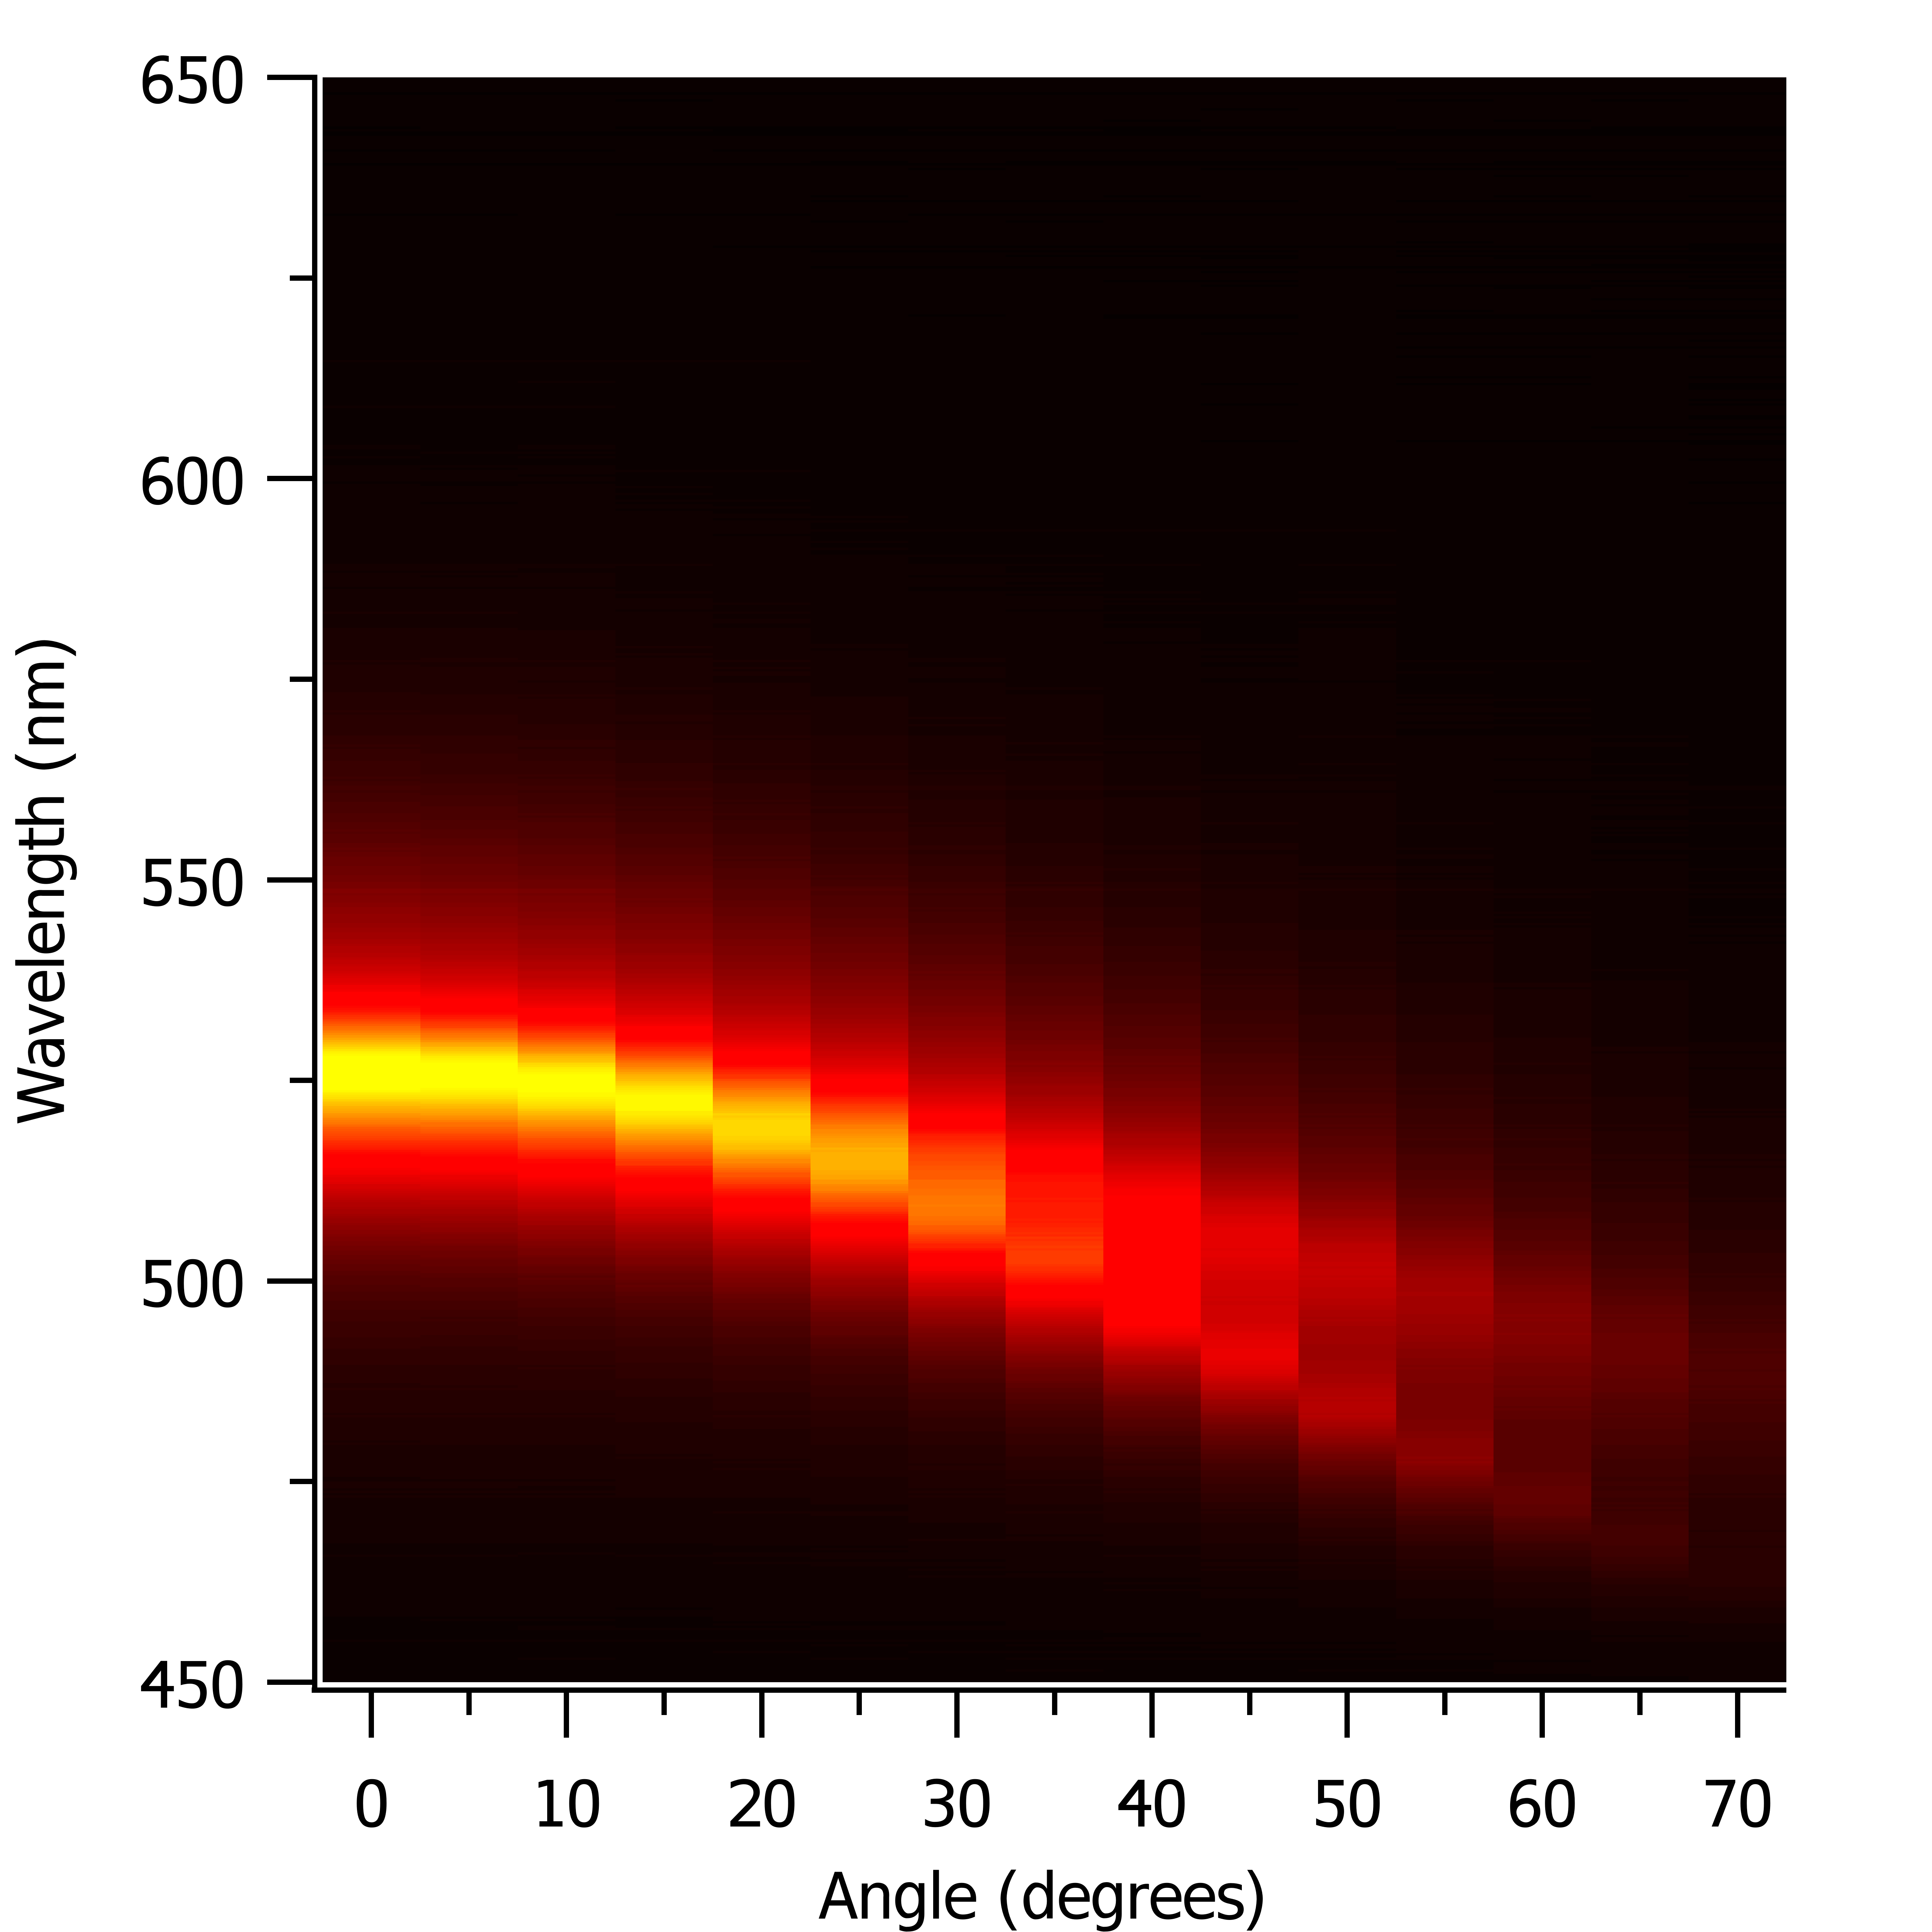
\includegraphics[width=0.45\textwidth]{images/n2_heatmap.png}
            (b)
            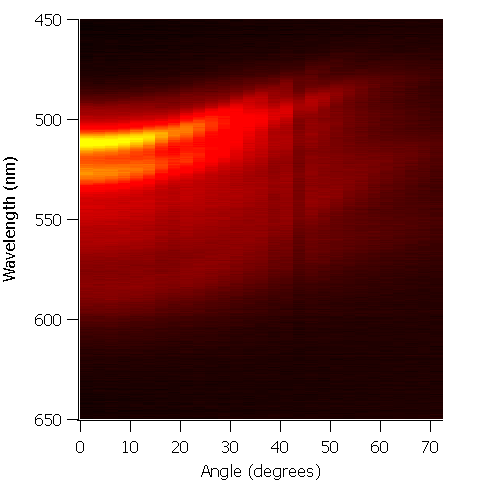
\includegraphics[width=0.45\textwidth]{images/n3_heatmap.png}
            \newline
            (c)
            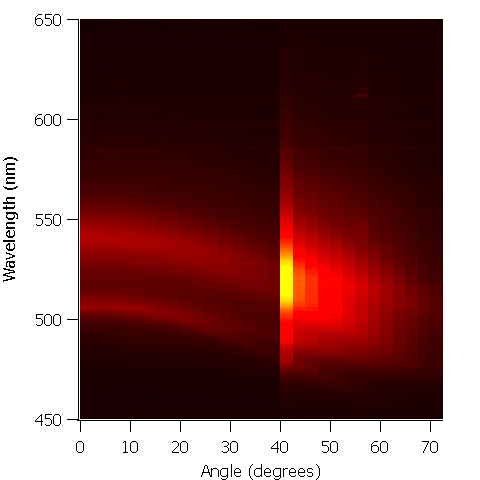
\includegraphics[width=0.45\textwidth]{images/n4_heatmap.png}
            (d)
            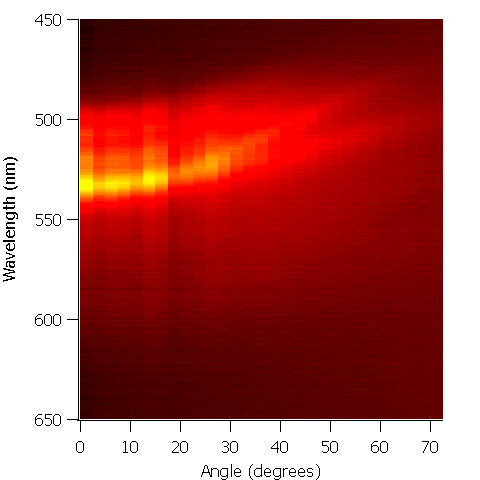
\includegraphics[width=0.45\textwidth]{images/n5_heatmap.png}
            \caption{Angular resolved emission profiles of devices with two (a), three (b), four (c), and five (d) cavities. The modal splitting of TE and TM modes can be seen along with the increase in emission modes at higher numbers of resonant cavities. The change in background intensity in the four cavity device (c) is due to a change in the iris size during data collection to maintain a strong signal.}
            \label{fig:heatmaps}
		\end{figure}
    
        \subsection{Behavior at Large Angles} \label{largeAngle}
		In the angular resolved emission spectroscopy, we see that the emission profile of the resonance cavities are highly dependent on the viewing angle. The peak emission blueshifts parabolically with increasing angle, and the emission splits into two distinctive peaks that separate as the angle increases. This is as would be predicted by the theory of wave propagation in a Fabry-P\'erot etalon (CITE doi:10.1021/es101052q). The modal splitting is the separation of the transverse electric (TE) and transverse magnetic (TM) modes splitting off from the superposition of them at $\theta=0$, called the transverse electric and magnetic (TEM) mode. (INCLUDE SOME MATH?)

    
        \subsection{Number of Resonant Modes} \label{numModes}
        We additinally see that a more complex modal structure can be generated with multi-cavity devices, even in forward emission. We see the first transition from one to two forward emission peaks in the transition from N=2 to N=3. The N=3 device has a narrow and intense emission peak at approximately 510nm with a slightly wider and weaker peak around 525nm. In the N=4 device, we also see two forward emission peaks, but the one around 510nm is significantly narrower and less intense with a broader, more intense peak occuring around 540nm. In the transition from N=4 to N=5, we see almost perfect preservation of the modal structure of N=4, with an additional peak superimposed between the two existing peaks. Although the cause of these additional peaks is not abundantly clear, the existence of two modes, one narrower than the other is logical. For example, in the N=4 device, the narrow peak could be generated by a resonant mode streching across the bottom three devices, while the broad peak is generated from resonances off of both the inner and outer interfaces of the top metal electrode. However, more experimentation would be necessary to confirm this theory.
        \begin{figure}[h!]
            \centering
            (a)
            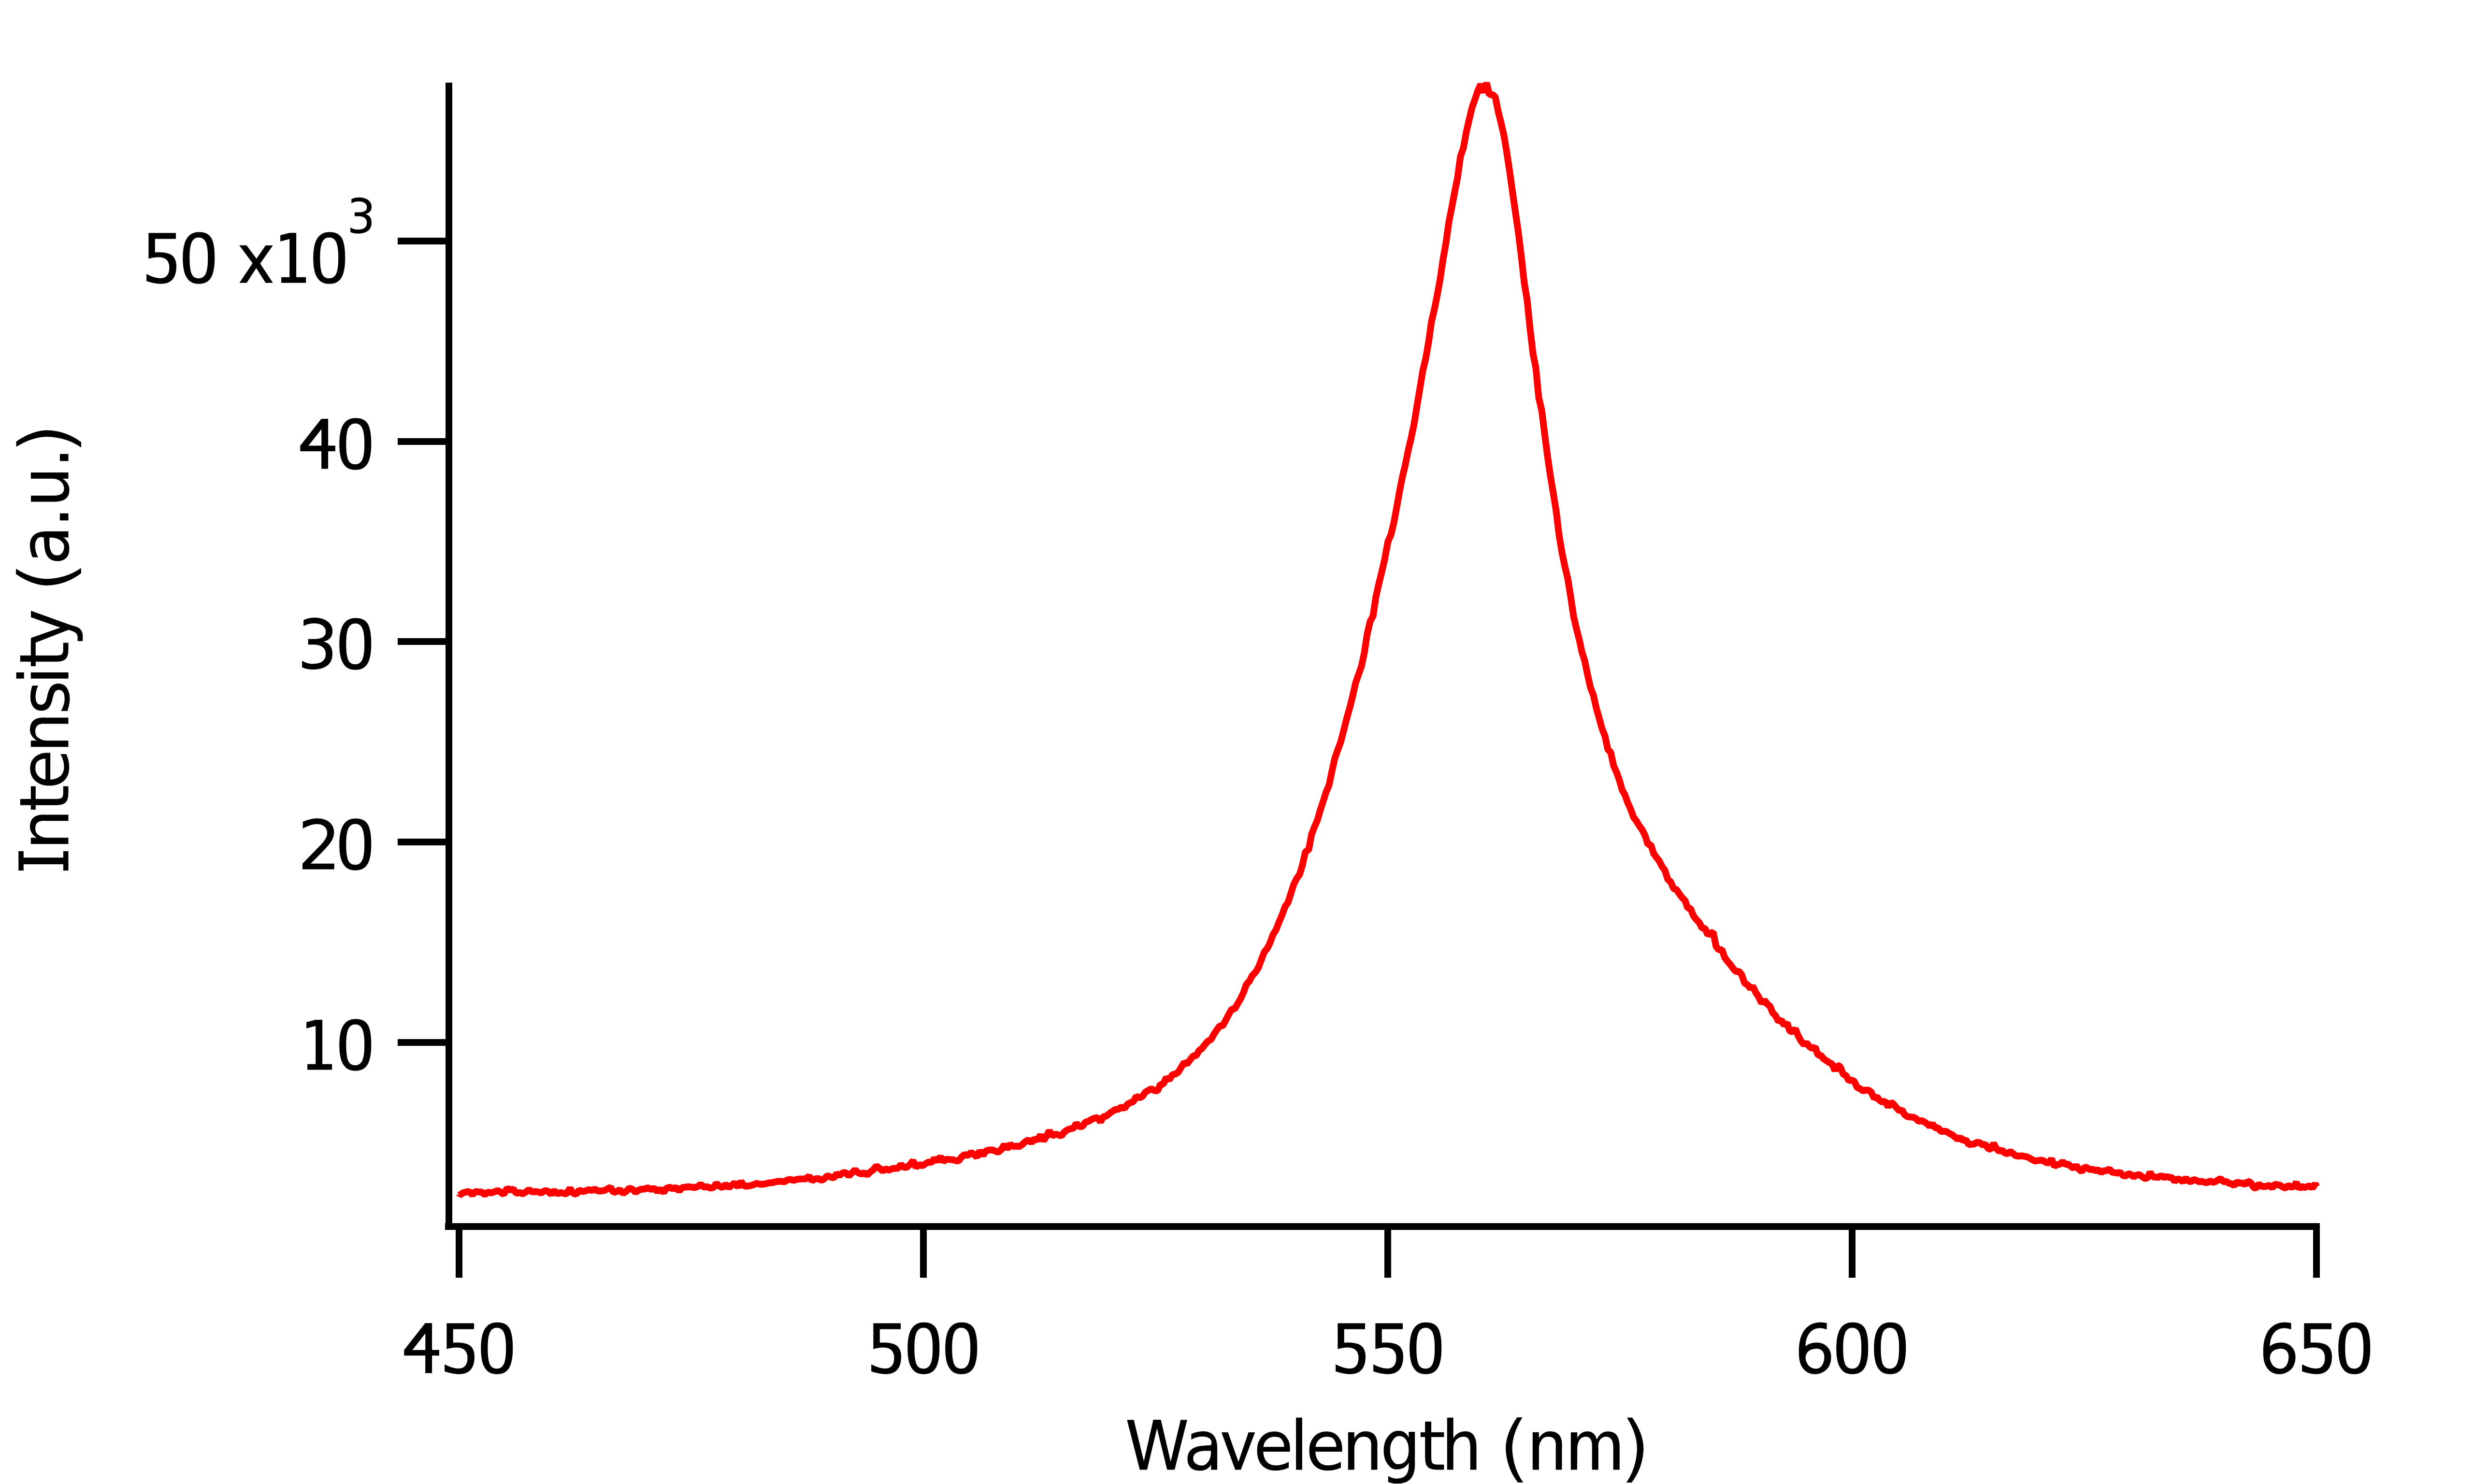
\includegraphics[width=0.45\textwidth]{images/n2_fe.png}
            (b)
            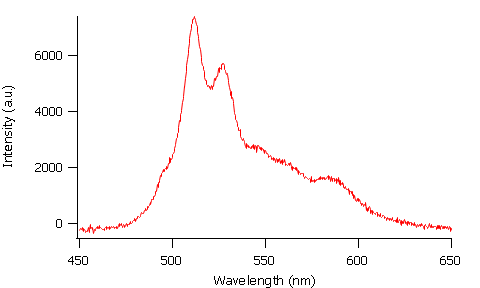
\includegraphics[width=0.45\textwidth]{images/n3_fe.png}
            \newline
            (c)
            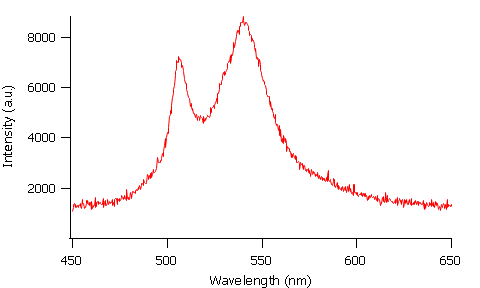
\includegraphics[width=0.45\textwidth]{images/n4_fe.png}
            (d)
            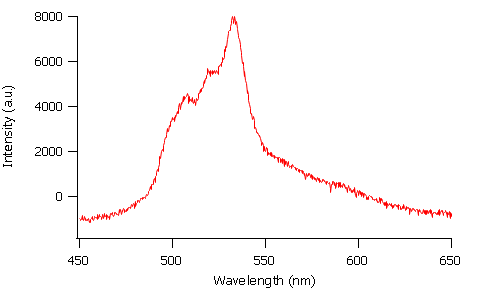
\includegraphics[width=0.45\textwidth]{images/n5_fe.png}
            \caption{Forward emission spectra of devices with two (a), three (b), four (c), and five (d) cavities. The transition from two to three cavities shows the introduction of an additional resonance mode, as does the transition from the four to the five cavity device. Additionally, the width of resonant peaks shrinks as more cavities are introduced.}
            \label{fig:fes}
        \end{figure}
        
        \subsection{Bandwidth of Resonant Modes} \label{modeWidth}

        By fitting with Lorentzian functions, the full width at half max (FWHM) can be found for each emission peak. By analyzing the FWHM for the emission peaks, we find a definite correlation that the emission bands narrow significantly as the number of cavities increases. This is expected for modes that form a resonant standing wave across several cavities for reasons similar to those presented in Section \ref{bandwidth}. As the number of cavities increases, the uncertainty in the position of a photon in the resonant mode increases, allowing for a more precise determination of its momentum, giving a narrower emission peak.
        \begin{figure}
            \centering
            \renewcommand{\arraystretch}{1.5}
            \setlength{\tabcolsep}{15pt}
            \begin{tabular}{|c|c|c|}
                \hline
                Number of Cavities & Peak Wavelength & Bandwidth \\
                \hline
                2 & 560nm & 19.77nm \\
                \hline
                3 & 512nm & 15.96nm \\
                  & 527nm & 17.25nm \\
                \hline
                4 & 507nm & 15.25nm \\
                  & 541nm & 15.91nm \\
                \hline
                5 & 533nm & 11.64nm \\
                \hline
            \end{tabular}

            \caption{Bandwidths of emission peaks in multi-cavity devices. Bandwidth is seen to shrink in all modes with the addition of another resonance cavity. Although three peaks exist in the N=5 device, only one peak is isolated enough to fit a reasonable Lorentzian to it.}
            \label{fwhm}
        \end{figure}


\chapter{Conclusion} \label{concl}

    In this project, we have demonstrated a technique for controlling the bandwidth and peak emission wavelength of an LED device, as well as generating more complex emission profiles. This technique utilizes device design and processing alone, rather than chemical changes to the actual materials. The linearity between peak wavelength and cavity thickness as well as the relationship between bandwidth and cavity thickness in single cavity devices allows for the ability to design and fabricate a device to match any desired single peak emission profile, provided  an emissive material with a sufficiently wide broadband emission spectrum is used. However, the same level of control can not yet be exerted over the complex emission spectra of multi-cavity devices.
    
    In the future, we hope to study the multicavity emission in more detail. In particular, a collection of emission spectra from multi-cavity devices with a different cavity thickness could contribute to a better understanding of the relationship of the emission peaks. Additionally, polarization analysis of the emission spectra of multi-cavity devices could lead to a stronger understanding of the modal structure of these devices.
    %In particular, a study of multi-cavity emission with varying thickness could yield a better understanding of the significance of the various emission peaks. Additionally, a polarization analysis of the emission profiles at large angles could contribute to a better understanding of the resonant cavity behavior.

\appendix
\chapter{Component Spectra of Angular Resolved Graphs} \label{components}

    \section*{Single Cavity Aluminum Topped Device}
    \begin{center}
    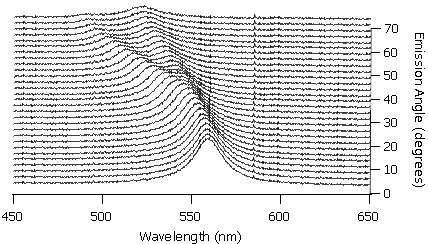
\includegraphics[width=0.95\textwidth]{images/n1_al_top_waterfall.png}
    \end{center}
    
    \section*{Single Cavity Silver Topped Device}
    \begin{center}
    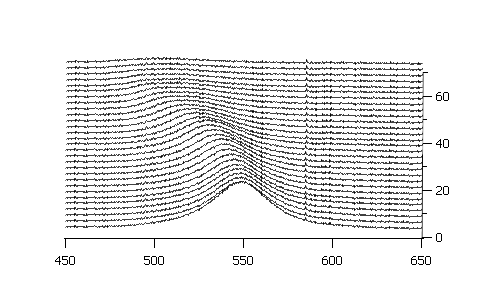
\includegraphics[width=0.95\textwidth]{images/n1_ag_top_waterfall.png}
    \end{center}
    
    \section*{Two Cavity Device}
    \begin{center}
    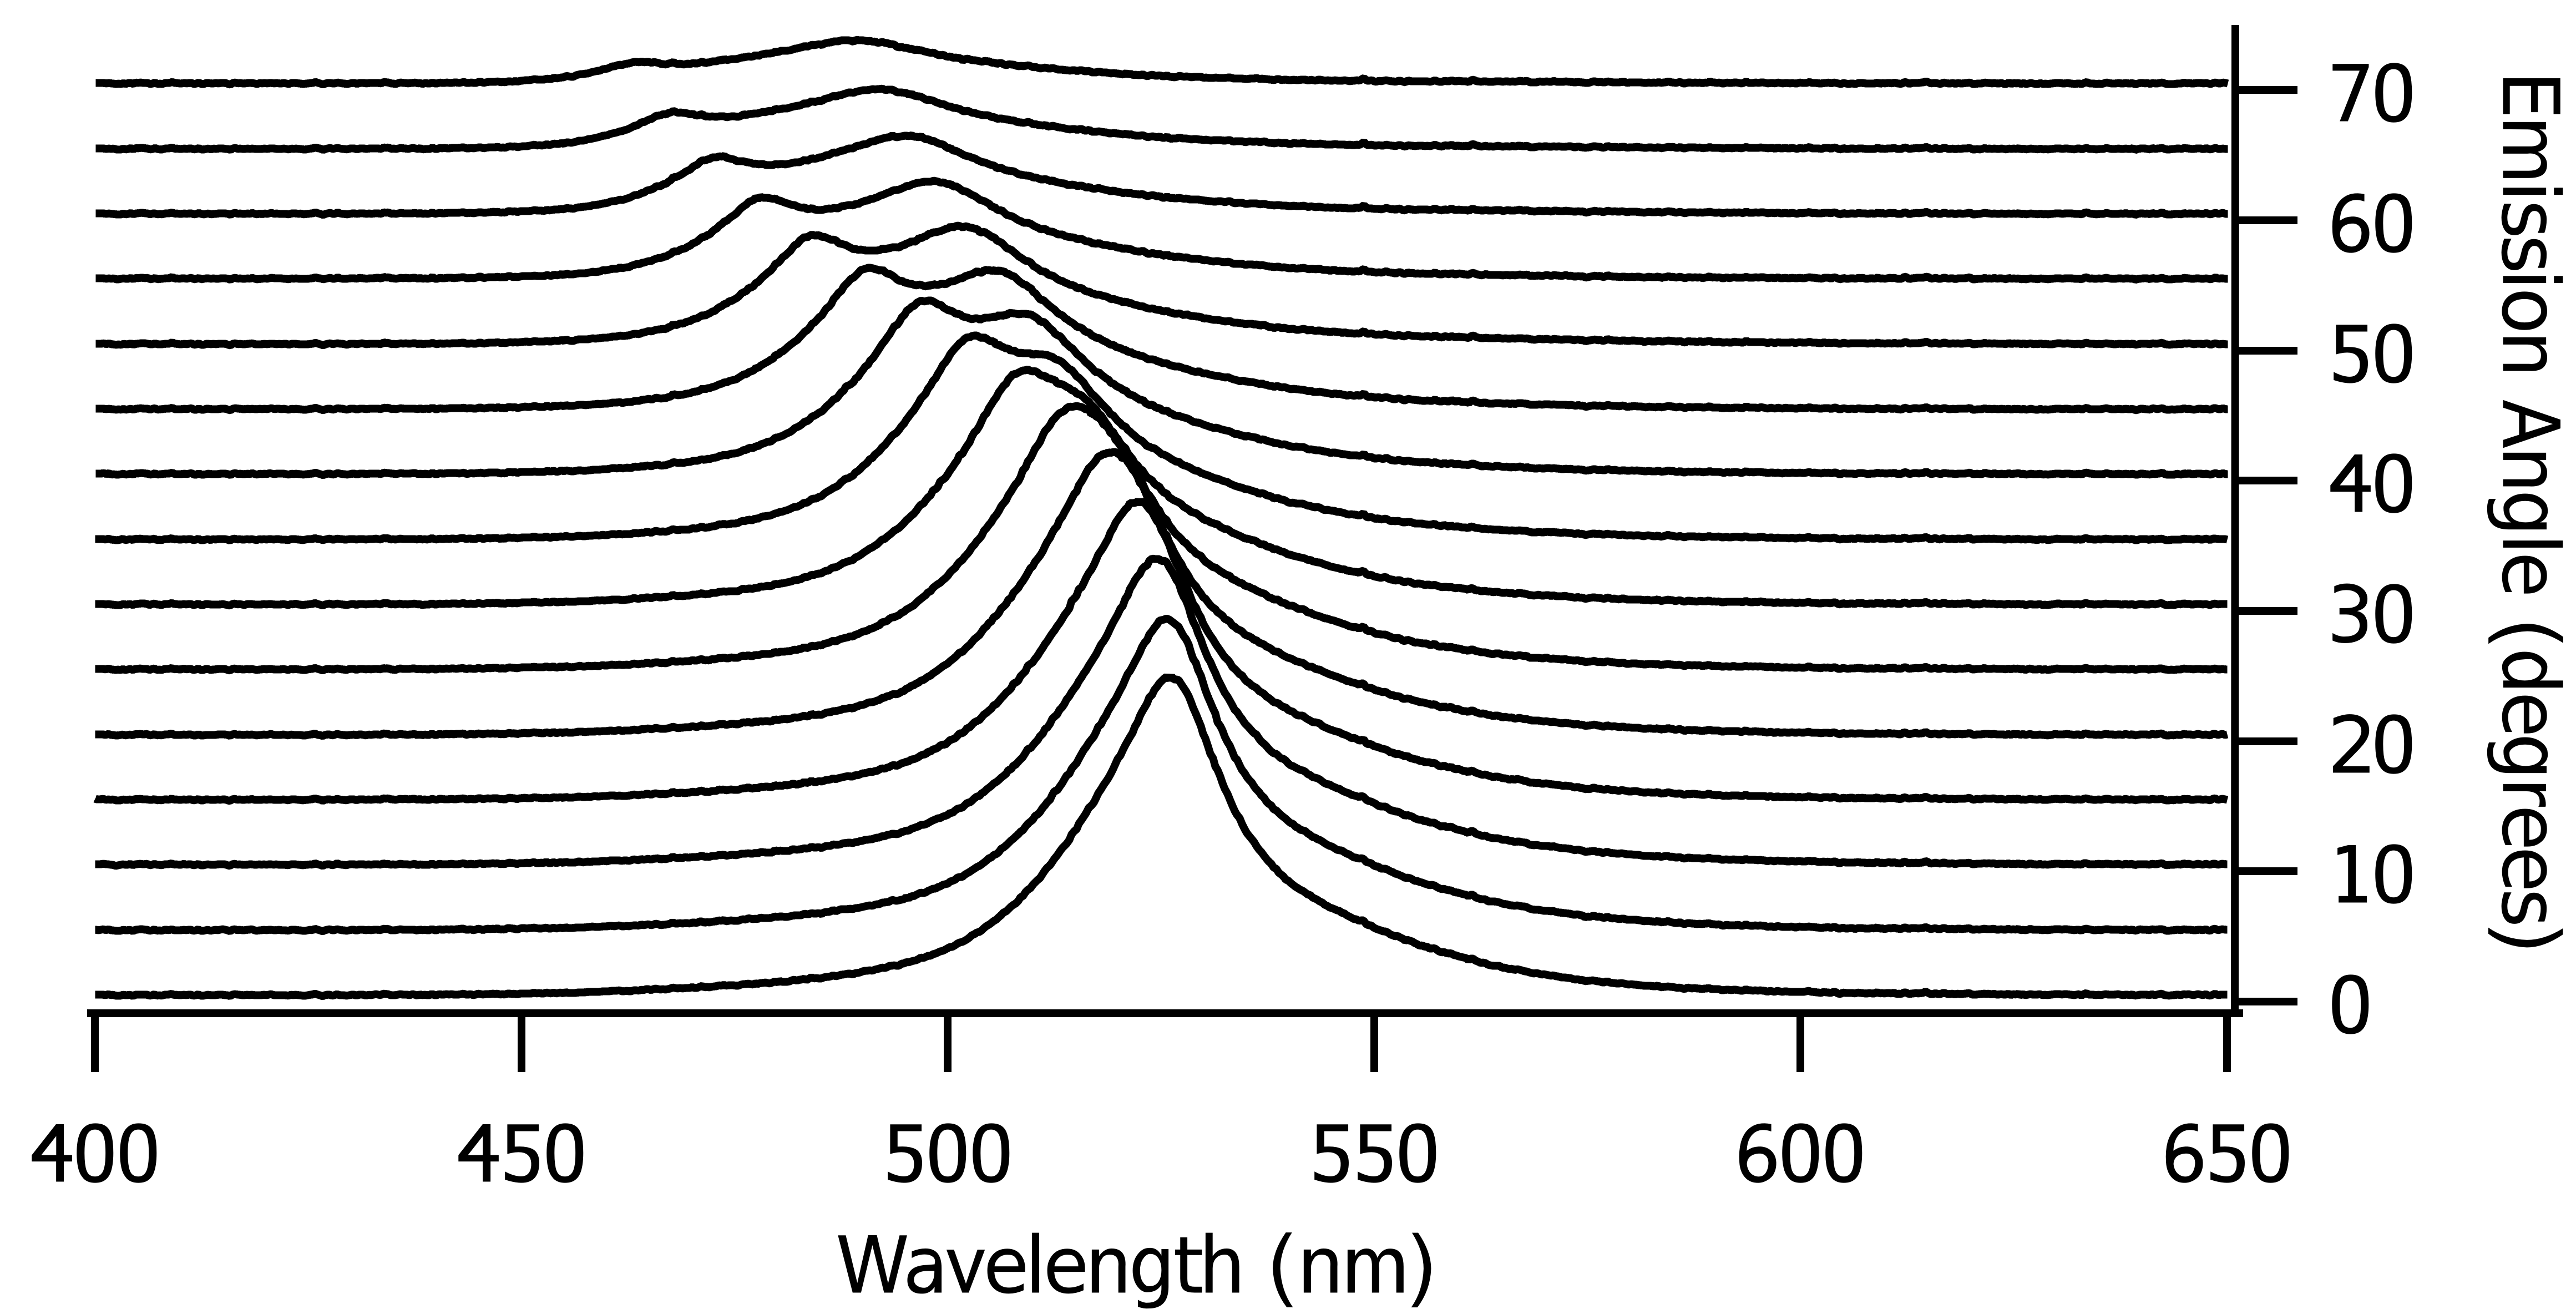
\includegraphics[width=0.95\textwidth]{images/n2_waterfall.png}
    \end{center}
    
    \section*{Three Cavity Device}
    \begin{center}
    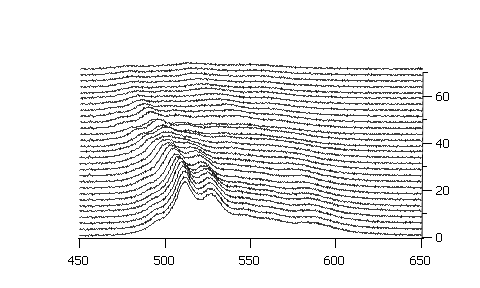
\includegraphics[width=0.95\textwidth]{images/n3_waterfall.png}
    \end{center}
    
    \section*{Four Cavity Device}
    \begin{center}
    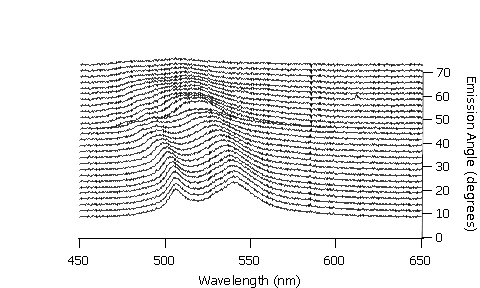
\includegraphics[width=0.95\textwidth]{images/n4_waterfall.png}
    \end{center}
    
    \section*{Five Cavity Device}
    \begin{center}
    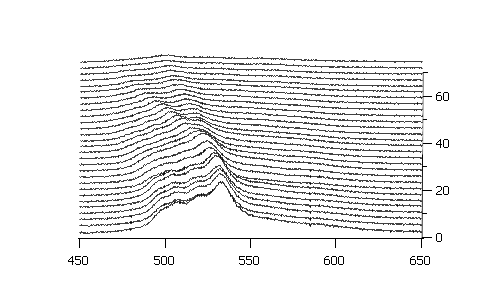
\includegraphics[width=0.95\textwidth]{images/n5_waterfall.png}
    \end{center}

\end{document}
